\chapter{Physical Implementation}


\section{Architecture}
The main specification we had to meet at all costs was to be able to take vector instructions as input, and output vector graphics on a screen. Roughly, our path through the process would go like this. 
\begin{enumerate}
\item Write the vector instructions in some self-defined format
\item Compile this format down to a bit-file
\item Feed the flash with this bit-file through the MCU, so we had the program stored in case of reboot. 
\item The (FPGA or MCU?) would read from this bit-file and translate it to instructions and store them in the SRAM. This would only happen once to load the entire initial program.
\item The FGPA would fetch these instructions from SRAM, execute them and the resulting graphic information would be stored in the frame buffer
\item Another part of the FPGA would simply send the information from the frame buffer to the DACs and HDMI
\item The output from the DACs would be displayed on an analogue oscilloscope and the output from the HDMI on a raster screen.
\end{enumerate}

\section{PCB Design}
The architecture was realized on a printed circuit board (PCB) that we designed using Altium Designer 15.1. We had never used this program before, and had to overcome the usual challenges and difficulties related to learning new software.

\subsection{Components}
The goal was to place the components so that they preferably were in close range of all other components they had to connect with. This would shorten the routing, which is desirable in terms of of mitigating signal delay and maintaining signal integrity.
\subsubsection{Main Components}
Our FPGA, SRAMs and MCU were the most important components with a lot of different connections, so we placed them very central on the PCB. Typical input and output stuff, e.g. controller buttons, USB, HDMI and BNC receptacles, were placed along the edge, since these are typically connected to few other components. It would also be annoying and unnecessary to connect external peripheral plugs to sockets in the middle of the PCB. 
\newline
The rest of our components were placed according to common sense. The DACs ended up between the FPGA and BNC connectors, voltage regulators close to power supply (USB), and so on. 
\subsubsection{Buttons and LEDS}
Buttons and LEDs, for use by the FPGA and the MCU, were placed near these components for simplicity. All buttons include a resistor for current limitation (to avoid short circuits) and pull-up (to avoid logical floating state). The exception is the button connected to the MCU, where the pin had internal pull-up. All LEDs also include a current limiting resistor. We calculated the required resistance using Ohm's law [insert citation].

\subsubsection{Decoupling Capacitors}
Several major components required decoupling, e.g. the MCU, FPGA, voltage regulators, and DACs. Decoupling means connecting power supplies through a capacitor network to ground, where power moving to ground can be temporarily stored. This was necessary because it sometimes occurs situations where there is suddenly high need for power. The power supply alone would not always be able to support these 'bursts'. A capacitor network was the solution to this problem, as the component could pull power from the capacitors instead.
\newline
It was important that this extra supply could reach the corresponding component as fast as possible. That's why all capacitors involved in the decoupling network for a certain component, were placed in close proximity to that component. All capacitors were placed on the bottom layer of the PCB to save space on an already crowded top layer.

\subsubsection{Component Footprints}
In the beginning, component footprints from the standard Altium library were used. After previewing the board, we saw that these footprints were in fact gigantic, and thus utilized Altium vaults to find smaller footprint sizes. We tried using the small 0603 (1608 metric) footprint for most of our passive components, especially the capacitors and resistors. By sticking to the same footprint, we could easily change our bill of materials without changing the PCB design, as long as the new component could be found in this package size. While a trade-off by using this small size package is that the components might be trickier to solder onto the board, the gain in size reduction for the board as a whole were valued higher by the group. Some components could not be found in this footprint, but luckily we had tons of other footprint sizes to choose from.


\subsection{Layers}
Our PCB consisted of six signal layers: Top layer, bottom layer and four in between. We had two power layers: VCC and ground.
\newline
Between every signal and power layer was a dielectric layer to make sure there was proper isolation between these conducting layers, so they didn't interfere with each other.
\newline
The bottom and top layer also had an overlay each. The overlay was there purely to contain silk-screen for marking components, thus making it easier for us to work with the PCB.
\newline
The complete layer stack is shown in figure \ref{fig:Layers}

\begin{figure}[h!]
\centering
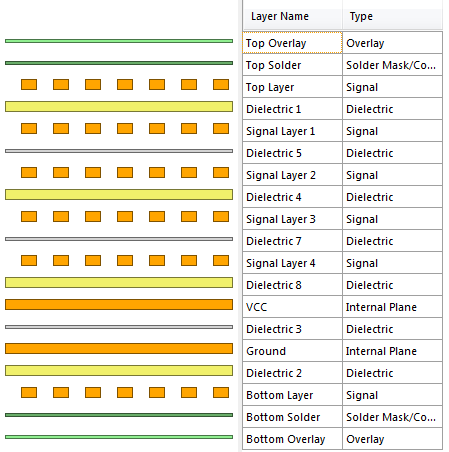
\includegraphics[scale = 0.8]{images/Layers.png}
\caption{Layer Stack}
\label{fig:Layers}
\end{figure}

\subsubsection{Power and ground}
Our PCB included three power domains, each with their corresponding voltage regulator: 3.3V, 1.2V and a 5V reserved for analogue signals. Most of our components were supplied by the 3.3V regulator, except for some internal parts of the FPGA that required 1.2V. Hence, we had to include this as a domain as well. 
\newline
\newline
Since 3.3V was used by most components, and since only a few connectors required 1.2V, we decided to have a dedicated power plane for 3.3V. We also had a dedicated ground plane. This saved us for yet more unnecessary routing, since everything connected to 3.3V or ground could go straight to a via by dogboning, and automatically be connected to the corresponding plane. The 1.2V traces were routed through all the connectors like any other signal. 

\subsubsection{Split planes}
The story of analogue 5V is a little different. The reason we had an analogue 5V, was to avoid noise from digital signals. The analogue components are sensitive to noise from the digital circuitry, and it was crucial for us to have as little noise as possible on the signal going to the oscilloscope. 
To avoid noise, the analogue and digital circuitry had to be separated completely. Analogue components could not use the same voltage supply as the digital ones and the same mattered for ground.
\newline
\newline
Our solution was to split the power and ground plane, shown in figure \ref{fig:Split planes}. 
\begin{itemize}
\item 5AV: Analogue 5V for components on the analogue plane. The reason it's 5V was because we weren't sure how much voltage the oscilloscope required to properly display the vector graphics from our program. 3.3V could be too low, so we went with 5V. Also, a high signal voltage could potentially help reduce noise.
\item AGND: Analogue components are connected to this ground instead of digital ground. This is to stop the analogue signal from getting disturbed by the digital signals on the ground plane.
\item 3.3V: Digital voltage for digital components.
\item GND: Digital ground.
\end{itemize}
All analogue components were placed in the analogue plane and the opposite with digital components. The exception was the DACs, which acts as a bridge between the digital part and the analogue part. These were placed on the actual split, with the affected pins on the correct side.
\newline
To remove any digital noise that could potentially accumulate on the analog ground plane, a diode was placed between the two ground planes, letting current flow from the analogue part to the digital part, but not vice versa.

\begin{figure}[h!]
\centering
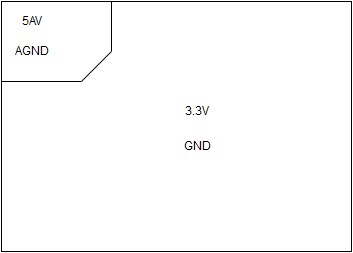
\includegraphics[scale = 0.6]{images/Split_planes.png}
\caption{Split between analogue and digital planes. The separating line is a solid, non-conducting material}
\label{fig:Split planes}
\end{figure}

\section{Routing}
Routing was a much more time-consuming process than we expected. We had put too much trust into the built-in auto router in Altium. The router did not, as we naively thought, magically solve the routing. 
\subsection{Design Rules}
Before routing, necessary rules had to be defined to make sure the PCB was routed properly. The following listing explains the most important rules for our design.
\begin{itemize}
\item Clearance: 0.1mm. 
\newline
Minimum clearance between different traces
\item Width: 0.127mm, Power Width 0.203mm.
\newline
Minimum width for traces. Power traces had bigger minimum widths, than signal traces.
\item Via Diameter: 0.4mm, Via Hole Size: 0.2mm
\newline
Minimum diameter and hole size for multi-layer vias.
\item Short-circuits and net antennas not allowed
\end{itemize}
The rules was set like this to make sure there wouldn't be any interference between traces, while the traces were still wide enough to not be damaged by the signal itself. Power traces were wider to make sure they could handle the voltage. 
\newline
Net antennas were traces that lead to dead-ends. This could harm the design, since these dead-ends could work as unwanted signal receivers from nearby sources.
\newline
\subsubsection{Design Rule Check}
Altium had its own tool for testing how many violations our current design created, called Design Rule Check. It displayed the amount of errors occurred from each type, and the coordinates on the PCB for every error. 
Typical errors during our design procedure was short-circuits, net antennas, clearance constraint violations, and so on.
\subsection{Routing Procedure}
First we started routing some components manually. We quickly discovered that doing this for the entire board would take a very long time, so we began to check out the built-in auto router in Altium. 
\newline
\newline
Roughly, we followed this routing procedure:
\begin{enumerate}
\item Run the auto router.
\item Run Design Rule Check, and see how many errors we get. 
\item If there are too many errors, like more than 200, there is most likely something wrong with our design rules, or the auto router settings. If not, go to step 6.
\item Check and modify settings and rules.
\item Go back to step 1.
\item Go through the remaining errors and fix them. 
\item ...
\item PROFIT!
\end{enumerate}
\subsection{Routing Problems}
We ran into many different routing problems, and we think it's important to address the major ones here for better understanding of how such problems arise.

\subsubsection{Bad Auto Router Settings}
After auto routing the whole thing the first time, the result was disappointing. It contained over 100 still unrouted connections, which means the auto router didn't manage to connect these.
\newline
\newline
We discovered that choosing different routing options for the auto router made a big difference. The default setting was \emph{Default 2 Layer Board}. Hence, the auto router focused on mainly using the top and bottom layer, and avoiding layer-switching. This resulted in the auto router not being able to route all the necessary connections.
\newline
\newline
After making the auto-router focus more on switching layers for every signals, to avoid complex routing on fewer layers, it managed to route all the connections. This was achieved by changing routing strategy from \emph{Default 2 Layer Board} to \emph{Default Multi Layer Board} in Altium.

\subsubsection{Clearance Constraint Issue}
After the first auto routing attempts, we got tons of short-circuits. We found out that our clearance constraint rule didn't apply for all components. The reason for this was a HDMI rule we had self-defined. The pads on the HDMI were placed so close together that we had to lower the clearance constraint for this component. To bypass this, we removed the general clearance constraint rule and instead made a new one to count for all traces, except for HDMI ones. This turned out to be a huge mistake, because now Altium couldn't find this general clearance constraint. This mistake lead to Altium not caring at all about clearances, thus routing as it pleased, which resulted in a short-circuit nightmare.
\newline
\newline
Adding the general clearance constraint rule back again, we faced the same issue in another form. The auto router wouldn't route at all, because it complained about clearance constraints violations. As frustrated as we were, since we thought we had just solved this, we had to start digging again. 
\newline
The clearance constraint rule was still the issue. The settings said that Altium would check for clearance violation with \emph{Any Net}. Thanks to some help from Odd Rune, we discovered that \emph{Any Net} also included the net that it was currently comparing. Thus, it checked if the current trace meets the clearance constraint with itself, which of course it does not. By changing this setting to \emph{Different Nets Only}, the entire short-circuit problem was solved. 

\subsubsection{Dead Copper}
Dead copper is parts of the copper on a power plane that's isolated from the rest of the copper on that plane. 
Dead copper appeared several places on our PCB. Normally it wasn't a problem, but some places a GND via or 3.3V via was connected to dead copper on the corresponding power plane. This wasn't desirable for the PCB, since we weren't sure what could happen then. 
\newline
We had to avoid power vias connected to dead copper, so we located every position where this situation occurred, and repositioned neighboring vias to rejoin the copper area with the main copper plane. The issue and solution are described in figure \ref{fig:Dead copper}.

\begin{figure}[h!]
\centering
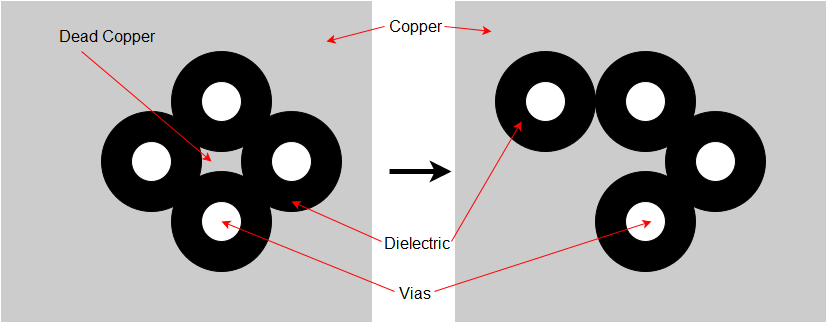
\includegraphics[scale = 0.4]{images/Dead_Copper.png}
\caption{Dead Copper. To the right, dead copper is avoided by moving one via}
\label{fig:Dead copper}
\end{figure}

\section{Redundancy}
We were inexperienced with PCB design and often uncertain if we had done something the right way, or misunderstood something. Our top priority was to make something that did work properly. A failing component was not unusual, and forgetting something was almost guaranteed to happen, considering the vast amount of factors involved. Hence, having back-up features was critical to us.
\subsection{Headers}
Our primary strategy of redundancy was including headers. A lot of headers. Our final amount of headers ended up at 34, including the JTAG and the ARM programming header. This would make us able to measure most signals with a multimeter and verify them. 
\newline
Pretty much every header was between components. If wrong connections existed, or a connection didn't work, we could use headers to easily correct the connections, by soldering on wires. Not only could we detect errors, but also fix them.

\begin{figure}[h!]
\centering
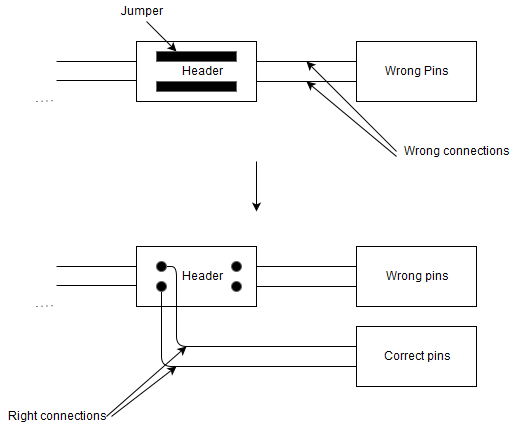
\includegraphics[scale = 0.45]{images/Header_fix.png}
\caption{Example Header fix}
\label{fig:Header fix}
\end{figure}

Headers was also useful as switches. By manually connecting header pins with jumpers, we could activate and deactivate certain parts of the PCB. This would be useful when focusing on lesser parts of the circuit. For instance, we used 3-pin headers to give us the ability of manually turning on and off different voltage levels. We could also deliver power to the components directly through the headers, should any of the wiring be wrong.

\subsection{DACs}
Even though we had our own DACs for outputting analog voltage out to the BNC plug, there was still a risk that we could not get them to work at all. We had a back-up solution by also connecting the internal DACs in the MCU to the BNCs. One header for each BNC input was used, to manually control if we wanted to use the main DACs or the MCU DACs. This is described in figure \ref{fig:DAC headers}. There's one header each for the X and the Y signal to the oscilloscope. 

\begin{figure}[h!]
\centering
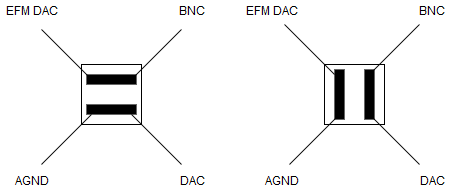
\includegraphics[scale = 0.6]{images/DAC_headers.png}
\caption{Left: Jumpers connecting MCU DAC to BNC and normal DAC to ground.
         Right: The opposite}
\label{fig:DAC headers}
\end{figure}

\section{Physical PCB and Components}
When we had received the PCB and the components, we had to make sure that every component worked properly independent of the PCB, then testing if they worked on the PCB. Many major components were impossible to test without soldering on the PCB though. Examples were the FPGA and MCU, because of their tiny ball grid pins.

\subsection{Soldering}
There were different ways of soldering components on the PCB. It depended on components being through hole, surface mounted, pin size, etc.
\subsubsection{Ball Grid Arrays (BGA)}
Both the FPGA and MCU were ball grid arrays.
Therefore, they were soldered on the PCB, by smearing paste over the corresponding area, putting them carefully on, and putting the PCB in a heater. The heater made the components stick properly to the paste. This was the only way, since soldering pins directly under the component by hand, isn't practically possible.

\subsubsection{Surface Mounted Components}
Most surface mounted components where the pins weren't too small and crowded, were soldered by hand. Paste were used before hand, just like with BGAs, but after that the pins could be soldered by hand, since the pins were within physical reach. 
\newline
If pins were too small and tight, the same technique was used as for the BGAs.

\subsubsection{Through Hole Components}
Through Hole components were the easiest to solder, since the pin size and the space between them was relatively large. Additionally they were on the bottom side of the board. No paste was needed, each individual pin could be soldered with tin wires.

\subsection{Testing}
We had to find and fix all errors and faults with our PCB design and components, that were a hazard to our desired resulting system.  
We ran tests during our soldering process to make sure the system so far worked desirably. Running tests during the process, lowered the amount of potential sources of errors, which made it easier to discover errors.

\subsubsection{Power Planes}
It was very important to verify that the power planes worked as we intended. Obviously, nothing would work without power. Hence, this was the very first test we performed.
\newline
Everything necessary for power to be present, was soldered on. This included power headers, and the 3.3 voltage regulator. External power was inserted through power headers. By measuring different places with a voltmeter, we already discovered anomalies. The voltmeter showed only 2.3V instead of 3.3V. Further testing revealed that one of the voltage regulator pins hadn't been soldered properly, resulting in a loss of 1V. After fixing this, the digital VCC plane contained the correct 3.3V.


\section{PCB Design Flaws}
No project would be complete without something going wrong. Our project is no exception. After receiving our manufactured PCB, we started to discover various complications. This section discusses the more serious ones in detail, and what we did to solve the problem.

\subsection{Incorrect Wiring}
We discovered that our buttons was wired wrong, since they caused short-circuits. The reason was sloppy study of the datasheet, as shown in figure \ref{fig:Button Issue}. Luckily, this could be remedied by rotating the button 90 degrees, if we adjusted the physical connectors to fit the footprint.

\begin{figure}[h!]
\centering
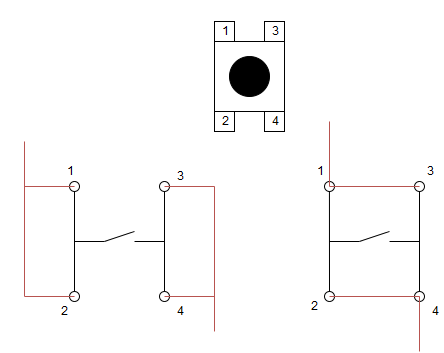
\includegraphics[scale=0.5]{images/Button_Issue.png}
\caption{Top figure shows the button as it looks like on the PCB. On the left: Correct wiring according to datasheet. On the right: Incorrect wiring leading to short-circuit}
\label{fig:Button Issue}
\end{figure}

When testing the oscillators, they did not seem to work. The datasheet for these components clearly stated that connecting the E/D pin to either 'No Connect' or '1' equaled active, so we did not connect it. We tried to remedy by connecting E/D to Vcc, and the problem was solved.
\newline
\newline
The Vref chip was supplied with 3.3V, but should have been supplied with analogue 5V instead. This could be remedied by cutting on the 3.3V power trace, since the trace is located on the top layer and no other traces are beneath it. Then we could connect analogue 5V via header from the voltage regulator to the input pin on the Vref chip.
\newline
The DACs were supplied with analogue 5V, but should have been supplied with 3.3V. The analogue 5V should go to the Vref chip instead. Solved by switching the two connections.

\subsection{PCB Placement and Footprints}
The BNC connector's footprint was wrongly routed - ground and Vcc was switched on the PCB. We discussed inverting the signal, but found that switching the pins on the component was the easiest thing to do.
\newline
\newline
It would have been beneficial if we had placed the 3.3V voltage regulator closer to the JTAG debugging port, since the Xilinx JTAG platform cable required a 3.3V power supply.
\newline
\newline
The micro USB footprint originally contained mounting holes, but were wrongly removed before manufacturing. Luckily, these did not act as connectors, and we could therefore solder the USB receptacle onto the PCB like a surface mount component.

\subsection{Component Order Issues}
The initial LEDs we ordered were reverse mounted, meaning that they required a hole in the board and had to be soldered on to the bottom layer. Because of this, we had to buy some new ones.
\newline
\newline

\subsection{Component sizes}
In hindsight, it would have been better to order bigger components. Since this is a prototype board where we mostly solder by hand, an increase in size would only be beneficial for us. If the project should go into large scale production, we could have tried to shrink the size.


